\begin{frame}
    \frametitle{\problemtitle}
    \begin{block}{Problem}
      Construct an $h\times w$ grid of the letters `\texttt{K}', `\texttt{I}' and `\texttt{T}' such that each letter occurs a given number of times and the word ``\texttt{KIT}'' appears exactly once when reading in the $8$ possible directions.
    \end{block}
    \centering
    
\includegraphics[width=0.35\textwidth]{sample-solved.pdf}
\end{frame}
\begin{frame}
    \frametitle{\problemtitle}
    \begin{block}{Solution}
      \begin{itemize}
        \item Start with ``\texttt{KIT}'' in the top left corner.
        \item Then place all the remaining `\texttt{T}'s, followed by all the `\texttt{K}'s and finally all the `\texttt{I}'s.
        \item No extra occurrences of ``\texttt{KIT}'' possible, as no `\texttt{I}' can be between a `\texttt{K}' and a `\texttt{T}'.
      \end{itemize}
    \end{block}
    \begin{center}
    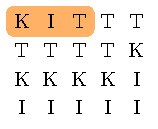
\includegraphics[width=0.3\textwidth]{sample-sorted-solved.pdf}
    \end{center}
    \pause
    \solvestats
\end{frame}
